\section*{Software Information}

\begin{itemize}
\item Please check, whether your inputs, the equations applied and the charactersitics are displayed correctly.
\item You are welcome to send your feedback via \url{https://github.com/oemof/tespy/issues}.
\item \LaTeX packages required are:
\begin{itemize}
\item graphicx
\item float
\item hyperref
\item booktabs
\item amsmath
\item units
\item cleveref
\end{itemize}
\item To supress these messages, call the model documentation with the keyword draft=False.
\end{itemize}

\begin{table}[H]
\begin{tabular}{ll}
TESPy Version:&0.4.3 - dev\\
Commit:&b8e11e11@dev\\
CoolProp version:&6.4.0\\
Python version:&3.7.6 (default, Jan  8 2020, 20:23:39) [MSC v.1916 64 bit (AMD64)]\\
Documentation generated:&Februar 24, 2021\\
\end{tabular}
\end{table}
\newpage\section{Connections in offdesign mode}

\subsection{Specified connection parameters}

\begin{table}[H]\begin{center}
\begin{tabular}{lrrr}
\toprule
                                              label &  p in $\unit[]{bar}$ (\ref{eq:Connection_pressure}) &  T in $\unit[]{^\circ C}$ (\ref{eq:Connection_temperature}) &  v in $\unitfrac[]{m3}{s}$ (\ref{eq:Connection_volumetric flow}) \\
\midrule
 consumer back flow:out1\_district heating pump:in1 &                                              10.000 &                                                      50.000 &                                                                - \\
                       condenser:out2\_consumer:in1 &                                                   - &                                                      90.000 &                                                                - \\
                         ambient air:out1\_pump:in1 &                                               1.000 &                                                       8.000 &                                                            0.167 \\
                     splitter:out1\_superheater:in1 &                                                   - &                                                           - &                                                            0.105 \\
                evaporator:out1\_sink ambient 1:in1 &                                               1.000 &                                                           - &                                                                - \\
\bottomrule
\end{tabular}
\caption{Specified connection parameters}
\end{center}\end{table}

\subsection{Equations applied}

\begin{equation}
\label{eq:Connection_pressure}
0 = p - p_\mathrm{spec}
\end{equation}

\begin{equation}
\label{eq:Connection_temperature}
0 = T \left(p, h \right) - T_\mathrm{spec}
\end{equation}

\begin{equation}
\label{eq:Connection_volumetric flow}
0 = \dot{m} \cdot v \left(p,h\right)- \dot{V}_\mathrm{spec}
\end{equation}

\subsection{Specified fluids}

\begin{table}[H]\begin{center}
\begin{tabular}{lrrr}
\toprule
                                              label &  NH3 (\ref{eq:Connection_NH3}) &  air (\ref{eq:Connection_air}) &  water (\ref{eq:Connection_water}) \\
\midrule
           coolant cycle closer:out1\_condenser:in1 &                          1.000 &                          0.000 &                              0.000 \\
 consumer back flow:out1\_district heating pump:in1 &                          0.000 &                          0.000 &                              1.000 \\
                         ambient air:out1\_pump:in1 &                          0.000 &                          0.000 &                              1.000 \\
\bottomrule
\end{tabular}
\caption{Specified fluids}
\end{center}\end{table}

\subsection{Equations applied}

\begin{equation}
\label{eq:Connection_NH3}
0 = x_\mathrm{NH3} - x_\mathrm{NH3,spec}
\end{equation}

\begin{equation}
\label{eq:Connection_air}
0 = x_\mathrm{air} - x_\mathrm{air,spec}
\end{equation}

\begin{equation}
\label{eq:Connection_water}
0 = x_\mathrm{water} - x_\mathrm{water,spec}
\end{equation}

\subsection{Referenced values for mass flow}

\begin{table}[H]\begin{center}
\begin{tabular}{llrr}
\toprule
                                             label &             reference &  factor in - &  delta in $\unitfrac[]{kg}{s}$ \\
\midrule
 evaporator reciculation pump:out1\_evaporator:in2 &  valve:out1\_drum:in1 &        1.250 &                              0 \\
\bottomrule
\end{tabular}
\caption{Referenced values for mass flow}
\end{center}\end{table}

\subsection{Equation applied}

\begin{equation}
\label{eq:Connection_ref}
0 = \text{value} - \text{value}_\mathrm{ref} \cdot \mathrm{factor} + \text{delta}
\end{equation}

\subsection{Referenced values for pressure}

\begin{table}[H]\begin{center}
\begin{tabular}{llrr}
\toprule
                                 label &                                           reference &  factor in - &  delta in $\unit[]{bar}$ \\
\midrule
 consumer:out1\_consumer feed flow:in1 &  consumer back flow:out1\_district heating pump:in1 &            1 &                        0 \\
\bottomrule
\end{tabular}
\caption{Referenced values for pressure}
\end{center}\end{table}

\subsection{Equation applied}

\begin{equation}
\label{eq:Connection_ref}
0 = \text{value} - \text{value}_\mathrm{ref} \cdot \mathrm{factor} + \text{delta}
\end{equation}

\subsection{Referenced values for enthalpy}

\begin{table}[H]\begin{center}
\begin{tabular}{llrr}
\toprule
                                 label &                                           reference &  factor in - &  delta in $\unitfrac[]{kJ}{kg}$ \\
\midrule
 consumer:out1\_consumer feed flow:in1 &  consumer back flow:out1\_district heating pump:in1 &            1 &                               0 \\
\bottomrule
\end{tabular}
\caption{Referenced values for enthalpy}
\end{center}\end{table}

\subsection{Equation applied}

\begin{equation}
\label{eq:Connection_ref}
0 = \text{value} - \text{value}_\mathrm{ref} \cdot \mathrm{factor} + \text{delta}
\end{equation}

\section{User defined equations in offdesign mode}

\section{Components in offdesign mode}

\subsection{Components of type CycleCloser}

\subsubsection{Mandatory constraints}

\begin{equation}
\label{eq:CycleCloser_pressure_equality_constraints}
0=p_{\mathrm{in,}i}-p_{\mathrm{out,}i}\; \forall i \in [1]
\end{equation}

\begin{equation}
\label{eq:CycleCloser_enthalpy_equality_constraints}
0=h_{\mathrm{in,}i}-h_{\mathrm{out,}i}\; \forall i \in [1]
\end{equation}


\subsection{Components of type Condenser}

\subsubsection{Mandatory constraints}

\begin{equation}
\label{eq:Condenser_mass_flow_constraints}
0=\dot{m}_{\mathrm{in,}i}-\dot{m}_{\mathrm{out,}i}\; \forall i \in [1, 2]
\end{equation}

\begin{equation}
\label{eq:Condenser_fluid_constraints}
0=x_{fl\mathrm{,in,}i}-x_{fl\mathrm{,out,}i}\;\forall fl \in\text{network fluids,}\; \forall i \in [1, 2]
\end{equation}

\begin{equation}
\label{eq:Condenser_energy_balance_constraints}
0 = \dot{m}_\mathrm{in,1} \cdot \left(h_\mathrm{out,1} - h_\mathrm{in,1} \right) +\dot{m}_\mathrm{in,2} \cdot \left(h_\mathrm{out,2} - h_\mathrm{in,2} \right)
\end{equation}


\subsubsection{Inputs specified}

\begin{table}[H]\begin{center}
\begin{tabular}{lrrll}
\toprule
     label &  pr1 (\ref{eq:Condenser_pr1}) &  zeta2 (\ref{eq:Condenser_zeta2}) &  kA\_char (\ref{eq:Condenser_kA_char}) &  subcooling (\ref{eq:Condenser_subcooling}) \\
\midrule
 condenser &                         0.990 &                         68800.601 &                                   True &                                        True \\
\bottomrule
\end{tabular}
\caption{Parameters of components of type Condenser}
\end{center}\end{table}

\subsubsection{Equations applied}

\begin{equation}
\label{eq:Condenser_pr1}
0=p_\mathrm{in,1}\cdot pr1 - p_\mathrm{out,1}
\end{equation}

\begin{equation}
\label{eq:Condenser_zeta2}
0 = \begin{cases}
p_\mathrm{in,2}- p_\mathrm{out,2} & |\dot{m}_\mathrm{in,2}| < \unitfrac[0.0001]{kg}{s} \\
\frac{\zeta}{D^4}-\frac{(p_\mathrm{in,2}-p_\mathrm{out,2})\cdot\pi^2}{8\cdot\dot{m}_\mathrm{in,2}\cdot|\dot{m}_\mathrm{in,2}|\cdot\frac{v_\mathrm{in,2} + v_\mathrm{out,2}}{2}}& |\dot{m}_\mathrm{in,2}| \geq \unitfrac[0.0001]{kg}{s}
\end{cases}
\end{equation}

\begin{equation}
\label{eq:Condenser_kA_char}
\begin{split}
0 = & \dot{m}_\mathrm{in,1} \cdot \left( h_\mathrm{out,1} - h_\mathrm{in,1}\right)\\
&+kA_\mathrm{design} \cdot f_\mathrm{kA} \cdot \frac{T_\mathrm{out,1} - T_\mathrm{in,2} - T_\mathrm{sat}\left( p_\mathrm{in,1}\right) +T_\mathrm{out,2}}{\ln{\frac{T_\mathrm{out,1}-T_\mathrm{in,2}}{T_\mathrm{sat}\left( p_\mathrm{in,1}\right)- T_\mathrm{out,2}}}}\\
f_\mathrm{kA}=&\frac{2}{\frac{1}{f\left(X_2\right)}+\frac{1}{f\left(X_2\right)}}\\
\end{split}
\end{equation}

\begin{equation}
\label{eq:Condenser_subcooling}
0=h_\mathrm{out,1} -h\left(p_\mathrm{out,1}, x=0 \right)
\end{equation}

\begin{minipage}{0.5\textwidth}
\begin{figure}[H]\begin{center}
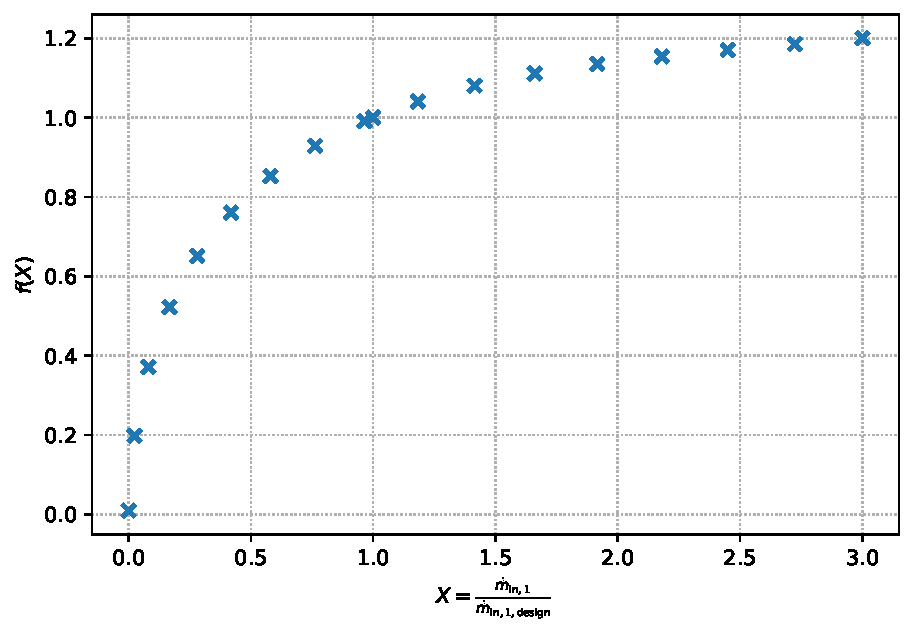
\includegraphics[width=\textwidth]{figures/Condenser_CharLine_kA_char1_condenser.pdf}
\caption{Characteristics of condenser (eq. \ref{eq:Condenser_kA_char})}
\label{fig:CharLine_kA_char1_condenser}
\end{center}\end{figure}

\end{minipage}
\begin{minipage}{0.5\textwidth}
\begin{figure}[H]\begin{center}
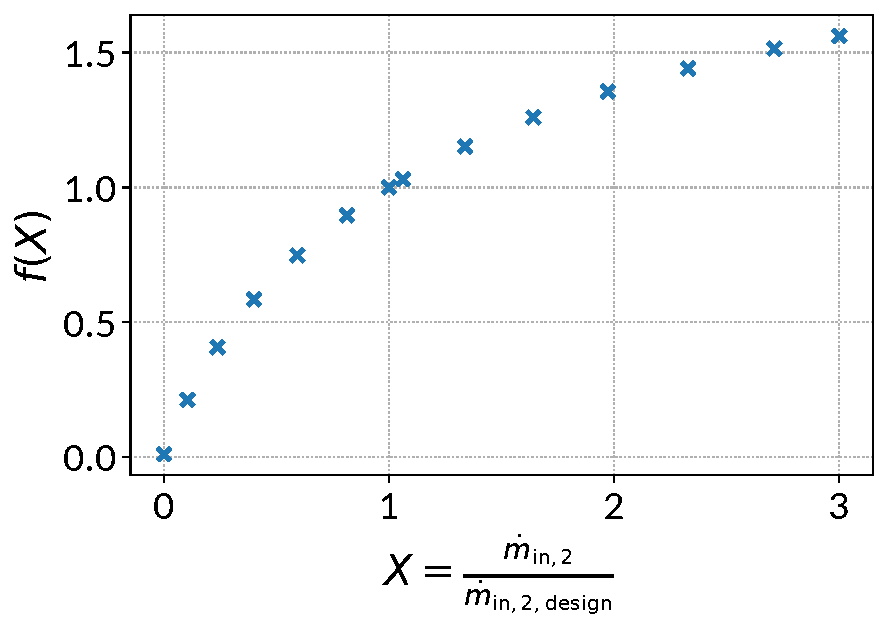
\includegraphics[width=\textwidth]{figures/Condenser_CharLine_kA_char2_condenser.pdf}
\caption{Characteristics of condenser (eq. \ref{eq:Condenser_kA_char})}
\label{fig:CharLine_kA_char2_condenser}
\end{center}\end{figure}

\end{minipage}


\subsection{Components of type Pump}

\subsubsection{Mandatory constraints}

\begin{equation}
\label{eq:Pump_mass_flow_constraints}
0=\dot{m}_{\mathrm{in,}i}-\dot{m}_{\mathrm{out,}i}\; \forall i \in [1]
\end{equation}

\begin{equation}
\label{eq:Pump_fluid_constraints}
0=x_{fl\mathrm{,in,}i}-x_{fl\mathrm{,out,}i}\;\forall fl \in\text{network fluids,}\; \forall i \in [1]
\end{equation}


\subsubsection{Inputs specified}

\begin{table}[H]\begin{center}
\begin{tabular}{ll}
\toprule
                        label &  eta\_s\_char (\ref{eq:Pump_eta_s_char}) \\
\midrule
        district heating pump &                                     True \\
 evaporator reciculation pump &                                     True \\
                         pump &                                     True \\
\bottomrule
\end{tabular}
\caption{Parameters of components of type Pump}
\end{center}\end{table}

\subsubsection{Equations applied}

\begin{equation}
\label{eq:Pump_eta_s_char}
0=\left(h_\mathrm{out}-h_\mathrm{in}\right)\cdot\eta_\mathrm{s,design}\cdot f\left( X \right)-\left( h_{out,s} - h_{in} \right)
\end{equation}

\begin{minipage}{0.5\textwidth}
\begin{figure}[H]\begin{center}
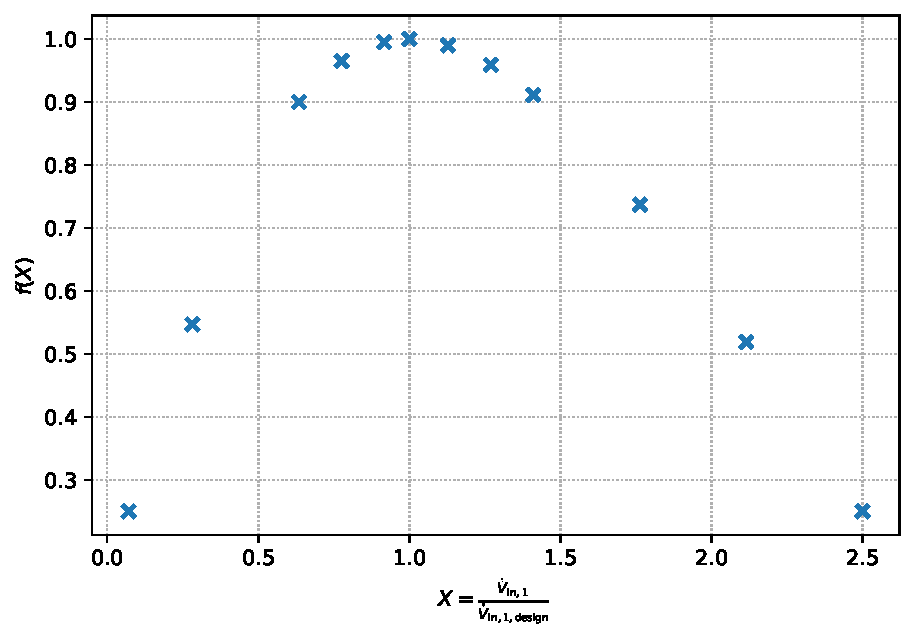
\includegraphics[width=\textwidth]{figures/Pump_CharLine_eta_s_char_district_heating_pump.pdf}
\caption{Characteristics of district heating pump (eq. \ref{eq:Pump_eta_s_char})}
\label{fig:CharLine_eta_s_char_district heating pump}
\end{center}\end{figure}

\end{minipage}
\begin{minipage}{0.5\textwidth}
\begin{figure}[H]\begin{center}
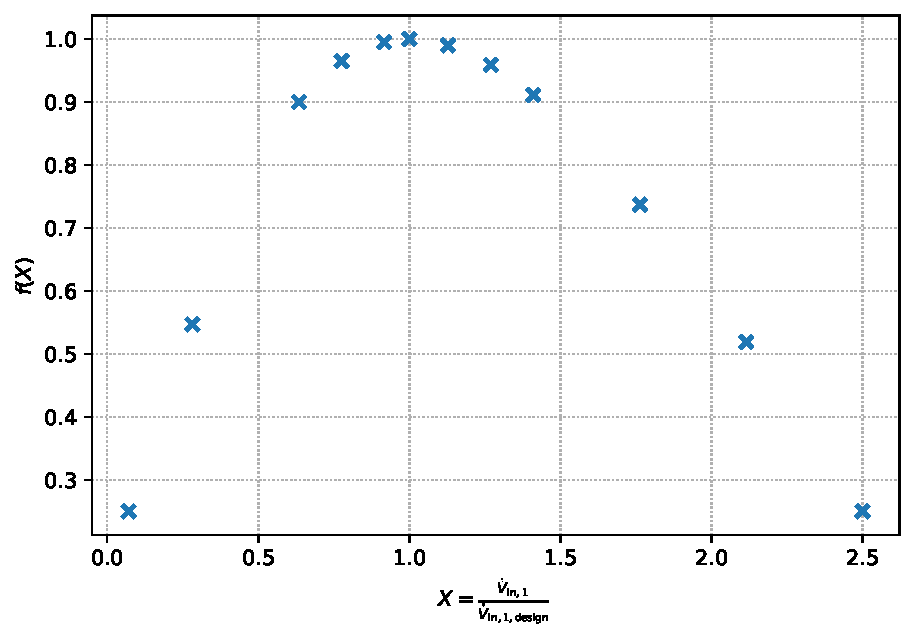
\includegraphics[width=\textwidth]{figures/Pump_CharLine_eta_s_char_evaporator_reciculation_pump.pdf}
\caption{Characteristics of evaporator reciculation pump (eq. \ref{eq:Pump_eta_s_char})}
\label{fig:CharLine_eta_s_char_evaporator reciculation pump}
\end{center}\end{figure}

\end{minipage}

\begin{minipage}{0.5\textwidth}
\begin{figure}[H]\begin{center}
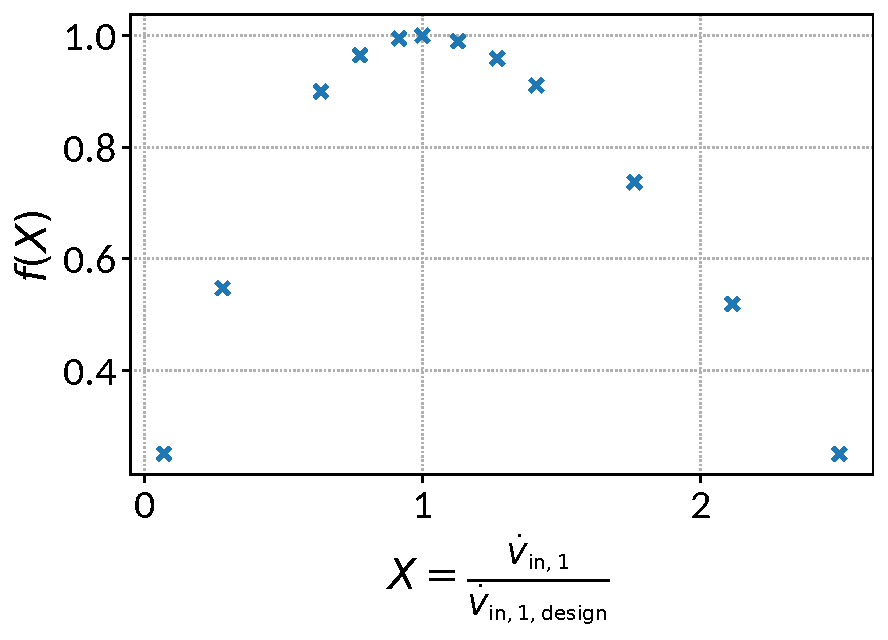
\includegraphics[width=\textwidth]{figures/Pump_CharLine_eta_s_char_pump.pdf}
\caption{Characteristics of pump (eq. \ref{eq:Pump_eta_s_char})}
\label{fig:CharLine_eta_s_char_pump}
\end{center}\end{figure}

\end{minipage}

\subsection{Components of type HeatExchangerSimple}

\subsubsection{Mandatory constraints}

\begin{equation}
\label{eq:HeatExchangerSimple_mass_flow_constraints}
0=\dot{m}_{\mathrm{in,}i}-\dot{m}_{\mathrm{out,}i}\; \forall i \in [1]
\end{equation}

\begin{equation}
\label{eq:HeatExchangerSimple_fluid_constraints}
0=x_{fl\mathrm{,in,}i}-x_{fl\mathrm{,out,}i}\;\forall fl \in\text{network fluids,}\; \forall i \in [1]
\end{equation}


\subsubsection{Inputs specified}

\begin{table}[H]\begin{center}
\begin{tabular}{lr}
\toprule
    label &  zeta (\ref{eq:HeatExchangerSimple_zeta}) \\
\midrule
 consumer &                                 68112.323 \\
\bottomrule
\end{tabular}
\caption{Parameters of components of type HeatExchangerSimple}
\end{center}\end{table}

\subsubsection{Equations applied}

\begin{equation}
\label{eq:HeatExchangerSimple_zeta}
0 = \begin{cases}
p_\mathrm{in,1}- p_\mathrm{out,1} & |\dot{m}_\mathrm{in,1}| < \unitfrac[0.0001]{kg}{s} \\
\frac{\zeta}{D^4}-\frac{(p_\mathrm{in,1}-p_\mathrm{out,1})\cdot\pi^2}{8\cdot\dot{m}_\mathrm{in,1}\cdot|\dot{m}_\mathrm{in,1}|\cdot\frac{v_\mathrm{in,1} + v_\mathrm{out,1}}{2}}& |\dot{m}_\mathrm{in,1}| \geq \unitfrac[0.0001]{kg}{s}
\end{cases}
\end{equation}


\subsection{Components of type Valve}

\subsubsection{Mandatory constraints}

\begin{equation}
\label{eq:Valve_mass_flow_constraints}
0=\dot{m}_{\mathrm{in,}i}-\dot{m}_{\mathrm{out,}i}\; \forall i \in [1]
\end{equation}

\begin{equation}
\label{eq:Valve_fluid_constraints}
0=x_{fl\mathrm{,in,}i}-x_{fl\mathrm{,out,}i}\;\forall fl \in\text{network fluids,}\; \forall i \in [1]
\end{equation}

\begin{equation}
\label{eq:Valve_enthalpy_equality_constraints}
0=h_{\mathrm{in,}i}-h_{\mathrm{out,}i}\; \forall i \in [1]
\end{equation}


\subsection{Components of type Drum}

\subsubsection{Mandatory constraints}

\begin{equation}
\label{eq:Drum_mass_flow_constraints}
0 =\sum\dot{m}_{\mathrm{in},i}-\sum\dot{m}_{\mathrm{out},j}\;\forall i \in \text{inlets}, \forall j \in \text{outlets}
\end{equation}

\begin{equation}
\label{eq:Drum_fluid_constraints}
0 = x_{fl\mathrm{,in,1}} - x_{fl\mathrm{,out,}j}\; \forall fl \in \text{network fluids,} \; \forall j \in\text{outlets}
\end{equation}

\begin{equation}
\label{eq:Drum_energy_balance_constraints}
0=\sum_i\left(\dot{m}_{\mathrm{in,}i}\cdot h_{\mathrm{in,}i}\right) - \sum_j \left(\dot{m}_{\mathrm{out,}j} \cdot h_{\mathrm{out,}j} \right) \; \forall i \in \text{inlets} \;\forall j \in \text{outlets}
\end{equation}

\begin{equation}
\label{eq:Drum_pressure_constraints}
\begin{split}
0 = p_\mathrm{in,1} - p_{\mathrm{in,}i} & \; \forall i \in \text{inlets} \setminus \left\lbrace 1\right\rbrace\\
0 = p_\mathrm{in,1} - p_{\mathrm{out,}j} & \; \forall j \in \text{outlets}\\
\end{split}
\end{equation}

\begin{equation}
\label{eq:Drum_outlet_constraints}
\begin{split}
0 =&h_\mathrm{out,1} -h\left(p_\mathrm{out,1}, x=0\right)\\0 =&h_\mathrm{out,2} -h\left(p_\mathrm{out,2}, x=1\right)\\\end{split}
\end{equation}


\subsection{Components of type HeatExchanger}

\subsubsection{Mandatory constraints}

\begin{equation}
\label{eq:HeatExchanger_mass_flow_constraints}
0=\dot{m}_{\mathrm{in,}i}-\dot{m}_{\mathrm{out,}i}\; \forall i \in [1, 2]
\end{equation}

\begin{equation}
\label{eq:HeatExchanger_fluid_constraints}
0=x_{fl\mathrm{,in,}i}-x_{fl\mathrm{,out,}i}\;\forall fl \in\text{network fluids,}\; \forall i \in [1, 2]
\end{equation}

\begin{equation}
\label{eq:HeatExchanger_energy_balance_constraints}
0 = \dot{m}_\mathrm{in,1} \cdot \left(h_\mathrm{out,1} - h_\mathrm{in,1} \right) +\dot{m}_\mathrm{in,2} \cdot \left(h_\mathrm{out,2} - h_\mathrm{in,2} \right)
\end{equation}


\subsubsection{Inputs specified}

\begin{table}[H]\begin{center}
\begin{tabular}{lrrrrl}
\toprule
       label &  kA (\ref{eq:HeatExchanger_kA}) &  pr2 (\ref{eq:HeatExchanger_pr2}) &  zeta1 (\ref{eq:HeatExchanger_zeta1}) &  zeta2 (\ref{eq:HeatExchanger_zeta2}) & kA\_char (\ref{eq:HeatExchanger_kA_char}) \\
\midrule
  evaporator &                               - &                             0.990 &                               227.824 &                                     - &                                      True \\
 superheater &                        9066.160 &                                 - &                               232.460 &                              3350.244 &                                         - \\
 intercooler &                               - &                                 - &                             56517.828 &                               680.633 &                                      True \\
\bottomrule
\end{tabular}
\caption{Parameters of components of type HeatExchanger}
\end{center}\end{table}

\subsubsection{Equations applied}

\begin{equation}
\label{eq:HeatExchanger_kA}
0 = \dot{m}_\mathrm{in,1} \cdot \left( h_\mathrm{out,1} - h_\mathrm{in,1}\right)+ kA \cdot \frac{T_\mathrm{out,1} - T_\mathrm{in,2} - T_\mathrm{in,1} + T_\mathrm{out,2}}{\ln{\frac{T_\mathrm{out,1} - T_\mathrm{in,2}}{T_\mathrm{in,1} - T_\mathrm{out,2}}}}
\end{equation}

\begin{equation}
\label{eq:HeatExchanger_pr2}
0=p_\mathrm{in,2}\cdot pr2 - p_\mathrm{out,2}
\end{equation}

\begin{equation}
\label{eq:HeatExchanger_zeta1}
0 = \begin{cases}
p_\mathrm{in,1}- p_\mathrm{out,1} & |\dot{m}_\mathrm{in,1}| < \unitfrac[0.0001]{kg}{s} \\
\frac{\zeta}{D^4}-\frac{(p_\mathrm{in,1}-p_\mathrm{out,1})\cdot\pi^2}{8\cdot\dot{m}_\mathrm{in,1}\cdot|\dot{m}_\mathrm{in,1}|\cdot\frac{v_\mathrm{in,1} + v_\mathrm{out,1}}{2}}& |\dot{m}_\mathrm{in,1}| \geq \unitfrac[0.0001]{kg}{s}
\end{cases}
\end{equation}

\begin{equation}
\label{eq:HeatExchanger_zeta2}
0 = \begin{cases}
p_\mathrm{in,2}- p_\mathrm{out,2} & |\dot{m}_\mathrm{in,2}| < \unitfrac[0.0001]{kg}{s} \\
\frac{\zeta}{D^4}-\frac{(p_\mathrm{in,2}-p_\mathrm{out,2})\cdot\pi^2}{8\cdot\dot{m}_\mathrm{in,2}\cdot|\dot{m}_\mathrm{in,2}|\cdot\frac{v_\mathrm{in,2} + v_\mathrm{out,2}}{2}}& |\dot{m}_\mathrm{in,2}| \geq \unitfrac[0.0001]{kg}{s}
\end{cases}
\end{equation}

\begin{equation}
\label{eq:HeatExchanger_kA_char}
\begin{split}
0 = & \dot{m}_\mathrm{in,1} \cdot \left( h_\mathrm{out,1} - h_\mathrm{in,1}\right)\\
&+kA_\mathrm{design} \cdot f_\mathrm{kA} \cdot \frac{T_\mathrm{out,1} - T_\mathrm{in,2} - T_\mathrm{in,1} + T_\mathrm{out,2}}{\ln{\frac{T_\mathrm{out,1} - T_\mathrm{in,2}}{T_\mathrm{in,1} - T_\mathrm{out,2}}}}\\
f_\mathrm{kA}=&\frac{2}{\frac{1}{f\left(X_1\right)}+\frac{1}{f\left(X_2\right)}}\\
\end{split}
\end{equation}

\begin{minipage}{0.5\textwidth}
\begin{figure}[H]\begin{center}
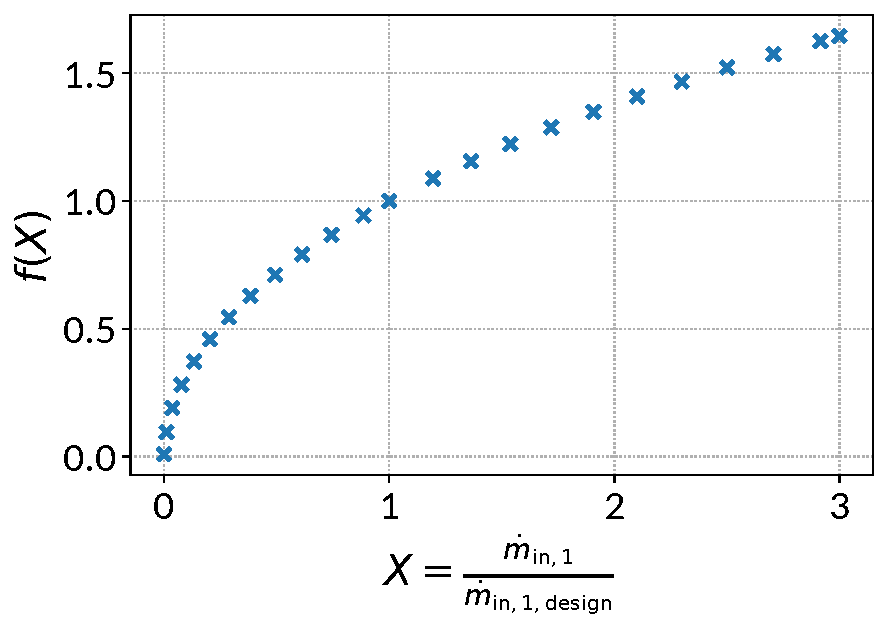
\includegraphics[width=\textwidth]{figures/HeatExchanger_CharLine_kA_char1_evaporator.pdf}
\caption{Characteristics of evaporator (eq. \ref{eq:HeatExchanger_kA_char})}
\label{fig:CharLine_kA_char1_evaporator}
\end{center}\end{figure}

\end{minipage}
\begin{minipage}{0.5\textwidth}
\begin{figure}[H]\begin{center}
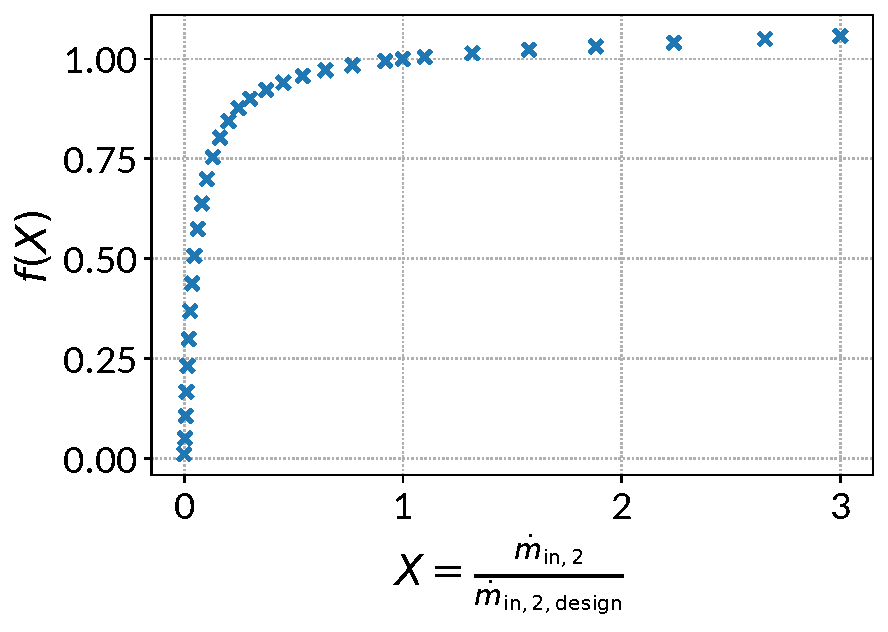
\includegraphics[width=\textwidth]{figures/HeatExchanger_CharLine_kA_char2_evaporator.pdf}
\caption{Characteristics of evaporator (eq. \ref{eq:HeatExchanger_kA_char})}
\label{fig:CharLine_kA_char2_evaporator}
\end{center}\end{figure}

\end{minipage}

\begin{minipage}{0.5\textwidth}
\begin{figure}[H]\begin{center}
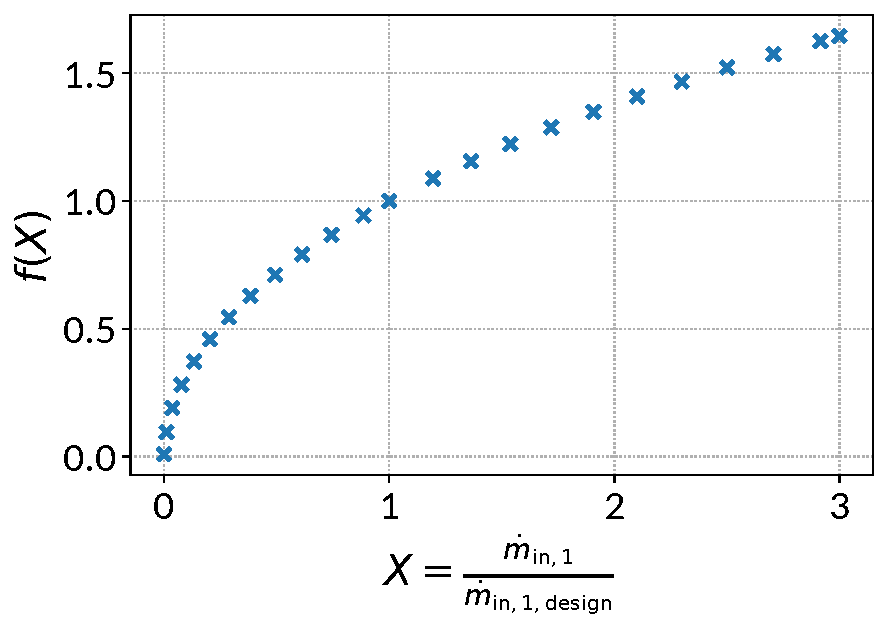
\includegraphics[width=\textwidth]{figures/HeatExchanger_CharLine_kA_char1_intercooler.pdf}
\caption{Characteristics of intercooler (eq. \ref{eq:HeatExchanger_kA_char})}
\label{fig:CharLine_kA_char1_intercooler}
\end{center}\end{figure}

\end{minipage}
\begin{minipage}{0.5\textwidth}
\begin{figure}[H]\begin{center}
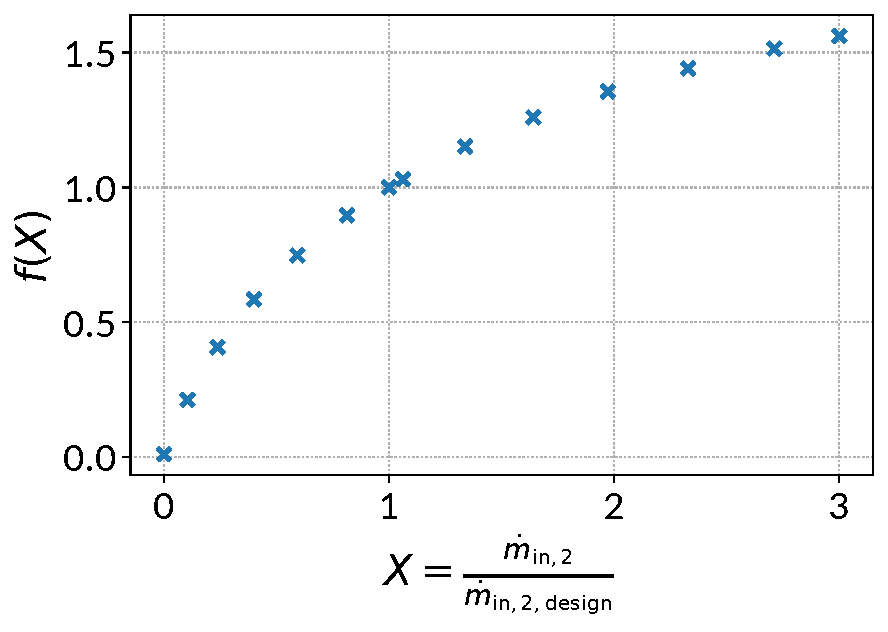
\includegraphics[width=\textwidth]{figures/HeatExchanger_CharLine_kA_char2_intercooler.pdf}
\caption{Characteristics of intercooler (eq. \ref{eq:HeatExchanger_kA_char})}
\label{fig:CharLine_kA_char2_intercooler}
\end{center}\end{figure}

\end{minipage}


\subsection{Components of type Splitter}

\subsubsection{Mandatory constraints}

\begin{equation}
\label{eq:Splitter_mass_flow_constraints}
0 =\sum\dot{m}_{\mathrm{in},i}-\sum\dot{m}_{\mathrm{out},j}\;\forall i \in \text{inlets}, \forall j \in \text{outlets}
\end{equation}

\begin{equation}
\label{eq:Splitter_fluid_constraints}
0 = x_{fl\mathrm{,in}} - x_{fl\mathrm{,out,}j}\; \forall fl \in \text{network fluids,} \; \forall j \in\text{outlets}
\end{equation}

\begin{equation}
\label{eq:Splitter_energy_balance_constraints}
0=h_{in}-h_{\mathrm{out,}j}\;\forall j \in\text{outlets}
\end{equation}

\begin{equation}
\label{eq:Splitter_pressure_constraints}
\begin{split}
0 = p_\mathrm{in,1} - p_{\mathrm{in,}i} & \; \forall i \in \text{inlets} \setminus \left\lbrace 1\right\rbrace\\
0 = p_\mathrm{in,1} - p_{\mathrm{out,}j} & \; \forall j \in \text{outlets}\\
\end{split}
\end{equation}


\subsection{Components of type Compressor}

\subsubsection{Mandatory constraints}

\begin{equation}
\label{eq:Compressor_mass_flow_constraints}
0=\dot{m}_{\mathrm{in,}i}-\dot{m}_{\mathrm{out,}i}\; \forall i \in [1]
\end{equation}

\begin{equation}
\label{eq:Compressor_fluid_constraints}
0=x_{fl\mathrm{,in,}i}-x_{fl\mathrm{,out,}i}\;\forall fl \in\text{network fluids,}\; \forall i \in [1]
\end{equation}


\subsubsection{Inputs specified}

\begin{table}[H]\begin{center}
\begin{tabular}{llr}
\toprule
        label &  eta\_s\_char (\ref{eq:Compressor_eta_s_char}) &  pr (\ref{eq:Compressor_pr}) \\
\midrule
 compressor 1 &                                           True &                            - \\
 compressor 2 &                                           True &                        3.000 \\
\bottomrule
\end{tabular}
\caption{Parameters of components of type Compressor}
\end{center}\end{table}

\subsubsection{Equations applied}

\begin{equation}
\label{eq:Compressor_eta_s_char}
0=\left(h_\mathrm{out}-h_\mathrm{in}\right)\cdot\eta_\mathrm{s,design}\cdot f\left(X\right)-\left( h_{out,s} - h_{in} \right)
\end{equation}

\begin{equation}
\label{eq:Compressor_pr}
0=p_\mathrm{in,1}\cdot pr - p_\mathrm{out,1}
\end{equation}

\begin{minipage}{0.5\textwidth}
\begin{figure}[H]\begin{center}
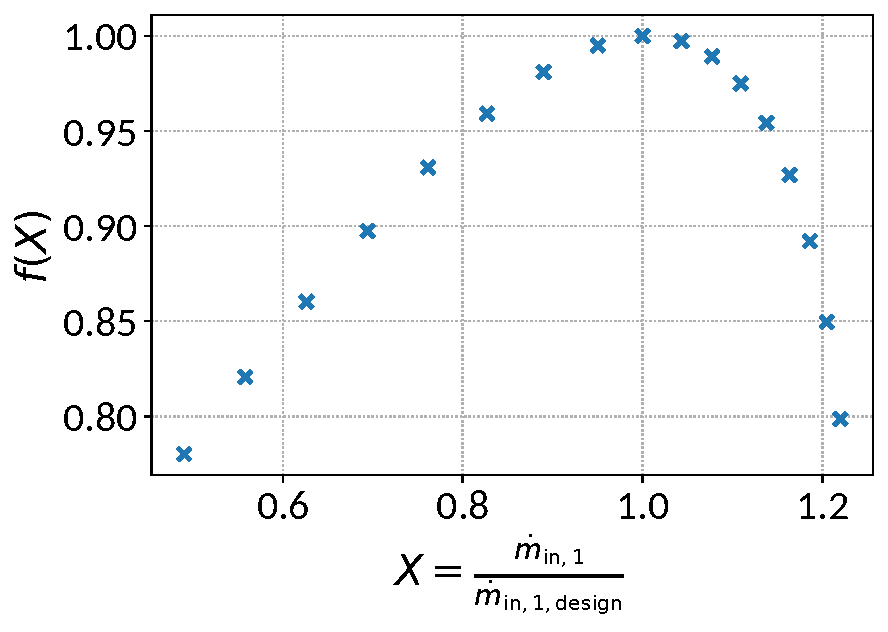
\includegraphics[width=\textwidth]{figures/Compressor_CharLine_eta_s_char_compressor_1.pdf}
\caption{Characteristics of compressor 1 (eq. \ref{eq:Compressor_eta_s_char})}
\label{fig:CharLine_eta_s_char_compressor 1}
\end{center}\end{figure}

\end{minipage}
\begin{minipage}{0.5\textwidth}
\begin{figure}[H]\begin{center}
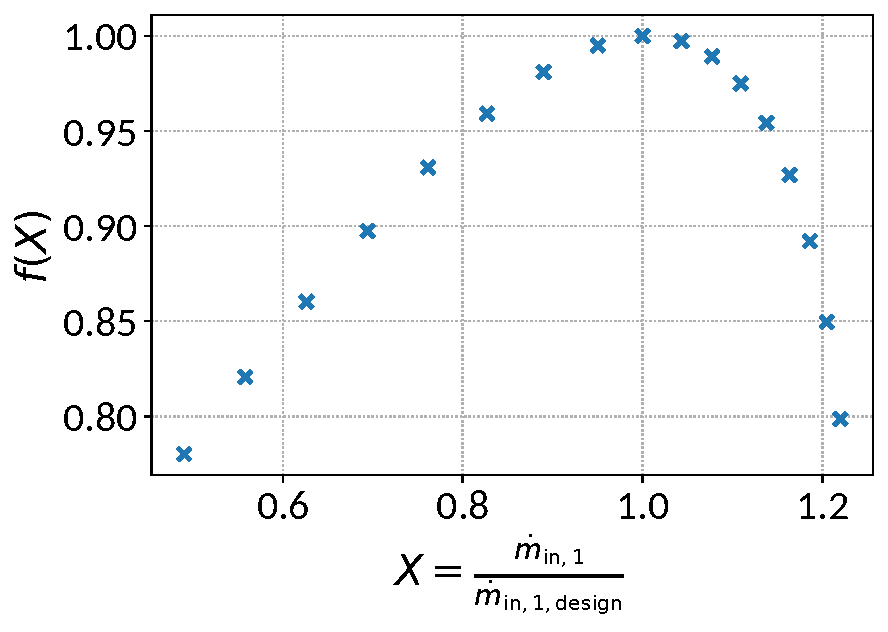
\includegraphics[width=\textwidth]{figures/Compressor_CharLine_eta_s_char_compressor_2.pdf}
\caption{Characteristics of compressor 2 (eq. \ref{eq:Compressor_eta_s_char})}
\label{fig:CharLine_eta_s_char_compressor 2}
\end{center}\end{figure}

\end{minipage}


\section{Busses in offdesign mode}

\subsection{Bus ``total compressor power''}

This bus is used for postprocessing only.

\begin{table}[H]\begin{center}
\begin{tabular}{llll}
\toprule
                        label &                                                   $\dot{E}_\mathrm{comp}$ &              $\dot{E}_\mathrm{bus}$ &                                                                            $\eta$ \\
\midrule
                 compressor 1 &  $\dot{m}_\mathrm{in} \cdot \left(h_\mathrm{out} - h_\mathrm{in} \right)$ &  $\dot{E}_\mathrm{comp} \cdot \eta$ &                  $f\left(X\right)$ (\ref{fig:Bus_CharLine_compressor 1offdesign}) \\
                 compressor 2 &  $\dot{m}_\mathrm{in} \cdot \left(h_\mathrm{out} - h_\mathrm{in} \right)$ &  $\dot{E}_\mathrm{comp} \cdot \eta$ &                  $f\left(X\right)$ (\ref{fig:Bus_CharLine_compressor 2offdesign}) \\
                         pump &  $\dot{m}_\mathrm{in} \cdot \left(h_\mathrm{out} - h_\mathrm{in} \right)$ &  $\dot{E}_\mathrm{comp} \cdot \eta$ &                          $f\left(X\right)$ (\ref{fig:Bus_CharLine_pumpoffdesign}) \\
        district heating pump &  $\dot{m}_\mathrm{in} \cdot \left(h_\mathrm{out} - h_\mathrm{in} \right)$ &  $\dot{E}_\mathrm{comp} \cdot \eta$ &         $f\left(X\right)$ (\ref{fig:Bus_CharLine_district heating pumpoffdesign}) \\
 evaporator reciculation pump &  $\dot{m}_\mathrm{in} \cdot \left(h_\mathrm{out} - h_\mathrm{in} \right)$ &  $\dot{E}_\mathrm{comp} \cdot \eta$ &  $f\left(X\right)$ (\ref{fig:Bus_CharLine_evaporator reciculation pumpoffdesign}) \\
\bottomrule
\end{tabular}
\caption{total compressor power}
\end{center}\end{table}



\begin{minipage}{0.5\textwidth}
\begin{figure}[H]\begin{center}
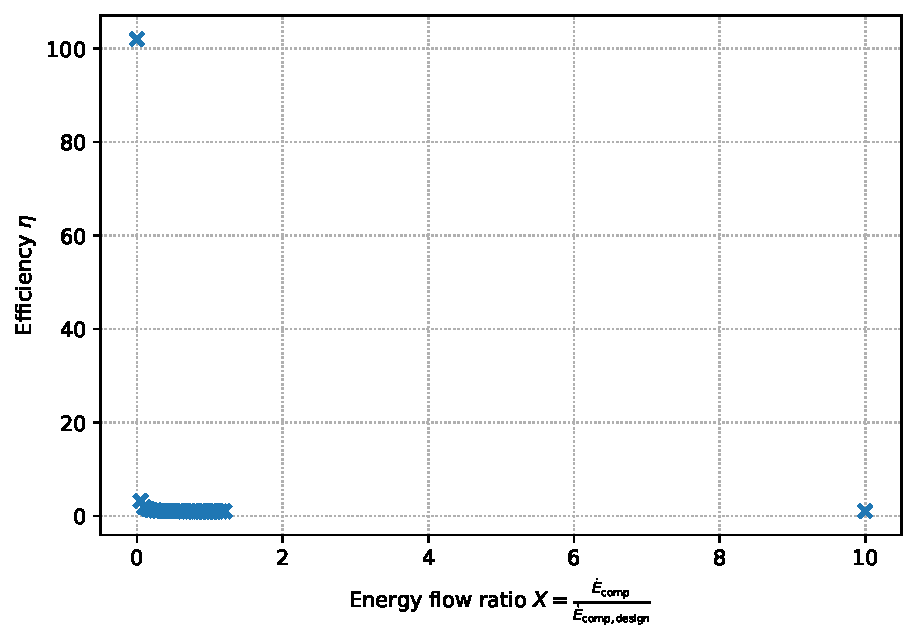
\includegraphics[width=\textwidth]{figures/Bus_CharLine_compressor_1offdesign.pdf}
\caption{Bus efficiency characteristic}
\label{fig:Bus_CharLine_compressor 1offdesign}
\end{center}\end{figure}

\end{minipage}
\begin{minipage}{0.5\textwidth}
\begin{figure}[H]\begin{center}
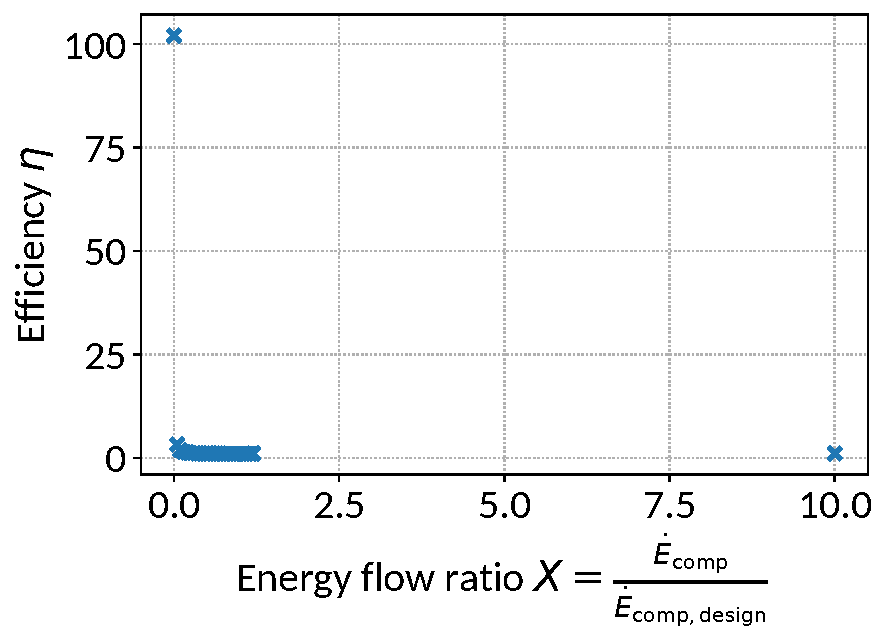
\includegraphics[width=\textwidth]{figures/Bus_CharLine_compressor_2offdesign.pdf}
\caption{Bus efficiency characteristic}
\label{fig:Bus_CharLine_compressor 2offdesign}
\end{center}\end{figure}

\end{minipage}

\begin{minipage}{0.5\textwidth}
\begin{figure}[H]\begin{center}
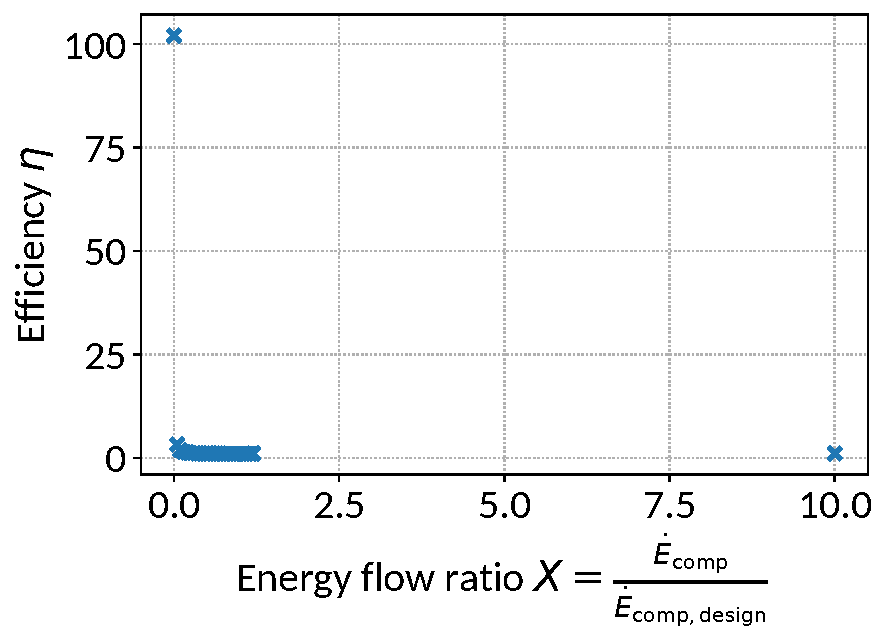
\includegraphics[width=\textwidth]{figures/Bus_CharLine_pumpoffdesign.pdf}
\caption{Bus efficiency characteristic}
\label{fig:Bus_CharLine_pumpoffdesign}
\end{center}\end{figure}

\end{minipage}
\begin{minipage}{0.5\textwidth}
\begin{figure}[H]\begin{center}
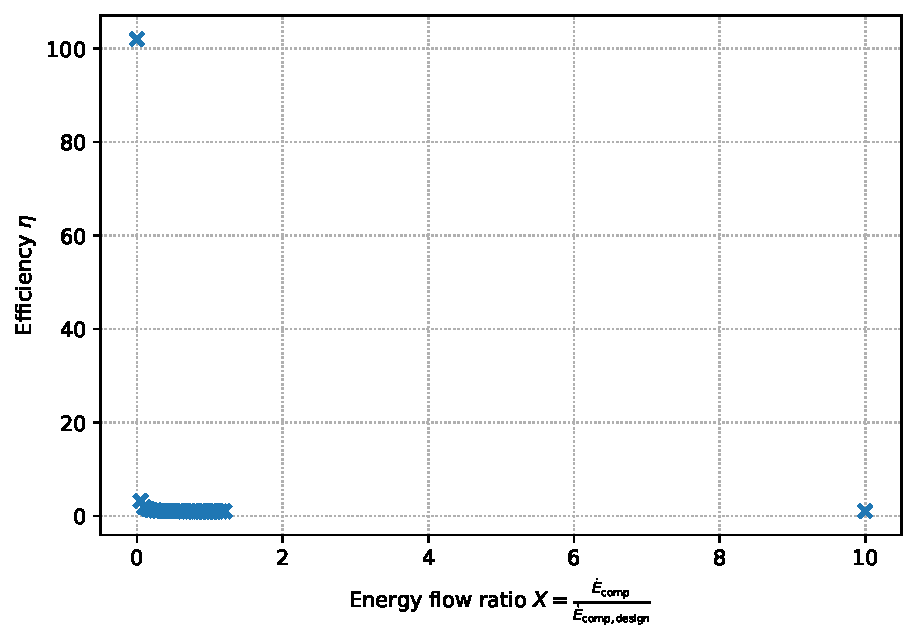
\includegraphics[width=\textwidth]{figures/Bus_CharLine_district_heating_pumpoffdesign.pdf}
\caption{Bus efficiency characteristic}
\label{fig:Bus_CharLine_district heating pumpoffdesign}
\end{center}\end{figure}

\end{minipage}

\begin{minipage}{0.5\textwidth}
\begin{figure}[H]\begin{center}
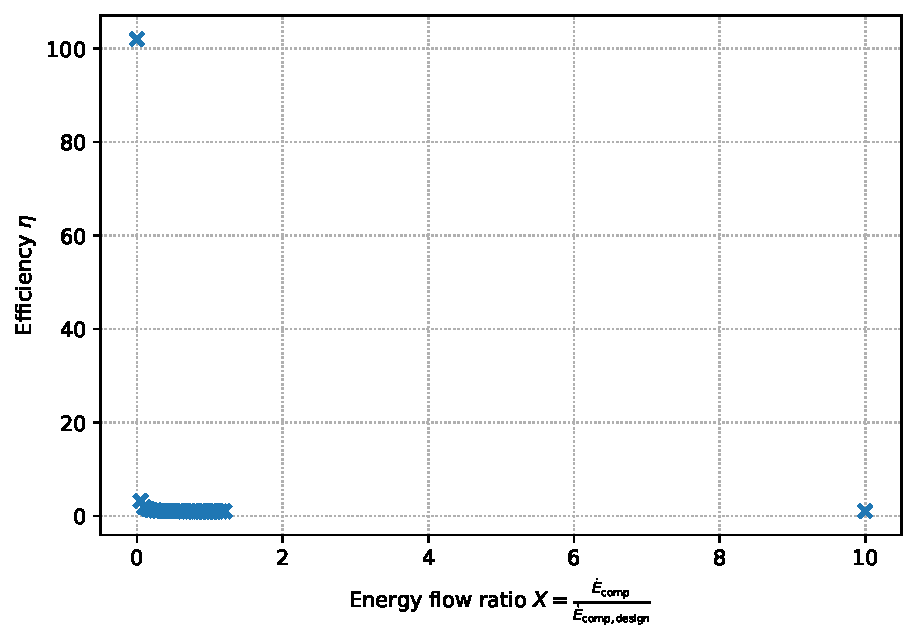
\includegraphics[width=\textwidth]{figures/Bus_CharLine_evaporator_reciculation_pumpoffdesign.pdf}
\caption{Bus efficiency characteristic}
\label{fig:Bus_CharLine_evaporator reciculation pumpoffdesign}
\end{center}\end{figure}

\end{minipage}

\subsection{Bus ``total delivered heat''}

Specified total value of energy flow: $\dot{E}_\mathrm{bus} = \unit[-2240000.000]{W}$

\begin{equation}
\label{eq:Bus_energy_flow_sum}
0=\dot{E}_\mathrm{bus} -\sum_i \dot{E}_{\mathrm{bus,}i}
\end{equation}

\begin{table}[H]\begin{center}
\begin{tabular}{llll}
\toprule
     label &                                                         $\dot{E}_\mathrm{comp}$ &              $\dot{E}_\mathrm{bus}$ & $\eta$ \\
\midrule
 condenser &  $\dot{m}_\mathrm{in,1} \cdot \left(h_\mathrm{out,1} - h_\mathrm{in,1} \right)$ &  $\dot{E}_\mathrm{comp} \cdot \eta$ &  1.000 \\
\bottomrule
\end{tabular}
\caption{total delivered heat}
\end{center}\end{table}




